\documentclass[10pt,a4paper]{scrartcl}
\usepackage[utf8]{inputenc}
\usepackage[francais]{babel}
\usepackage{lmodern}
\usepackage[T1]{fontenc}
\usepackage{xcolor}
\usepackage{graphicx}
\usepackage{amsmath, amssymb, amsthm}
\usepackage{geometry}
\usepackage{thmbox}
\usepackage{enumerate}
\usepackage{subcaption}

\geometry{
a4paper,
body={150mm,260mm},
left=30mm,top=15mm,
headheight=7mm,headsep=4mm,
marginparsep=4mm,
marginparwidth=27mm}

\pagestyle{empty}

\providecommand{\abs}[1]{\left|#1\right|}
\providecommand{\C}{\mathbb{C}}
\providecommand{\R}{\mathbb{R}}
\providecommand{\E}{\mathbb{E}}
\providecommand{\Prob}{\mathbb{P}}
\providecommand{\ii}{\mathrm{i}}
\providecommand{\w}{\omega}
\providecommand{\one}{\textbf{1}}

\renewcommand{\S}{\textbf{S}^n}

\newcommand{\norm}[1]{\Arrowvert#1\Arrowvert_2}

\newcount\colveccount

\newcommand*\colvec[1]{
        \global\colveccount#1
        \begin{pmatrix}
        \colvecnext
}
\def\colvecnext#1{
        #1
        \global\advance\colveccount-1
        \ifnum\colveccount>0
                \\
                \expandafter\colvecnext
        \else
                \end{pmatrix}
        \fi
}
 
\author{Judith Abecassis \& Timothée Lacroix}

\title{Random Graph Bandits with side information}


\begin{document}
\maketitle

\section{Introduction}
\subsection{Context}
We are interested in the multi-armed bandit with side information setting \cite{mannor2011bandits, alon2013bandits, kocak2014efficient}. This consists in a sequential learning where, at each iteration, the learner chooses an arm, and observes losses of a number of arms. This is a generalization of two well-studied feedback settings~\cite{cesa2006prediction}, one in which the learner only knows the loss of the arm it pulled (bandit setting), and the other where the losses of all arms are revealed (full information setting). Full information occurs for example for trading on a stock market: all stock prices are known, and the bandit setting can be illustrated by electronic advertising. A situation of partial revelation of other arms could be considered in advertising in a social network.

We are following the formalism previouly proposed by Mannor and Shamir (2011)~\cite{mannor2011bandits} in which side observations are modeled using a graph structure: each possible action is a node, and when an action is chosen, its loss and the losses of all its neighbours in the graph are revealed. Our work is in the line of Valko et al. (2015, under review), and considers the case where no previous information on the structure of the graph is known, and where partial observation is stochastic. 

We will be considering two models of random graphs.

\subsection{Different Graphs models}

\subsubsection{Erdos-Renyi}
Let $0\leq p \leq 1$. $E=ER(p)$ is the graph such that $(i \rightarrow j) \in E$ with probability $p$. Such graphs have very well understood properties. Their expected independence number $\bar{\alpha}$ is ????????.
Examples of ER graphs are given in Fig~\ref{er_ex}.

\begin{figure}[hh!]
\begin{center}
        \begin{subfigure}[b]{0.45\textwidth}
                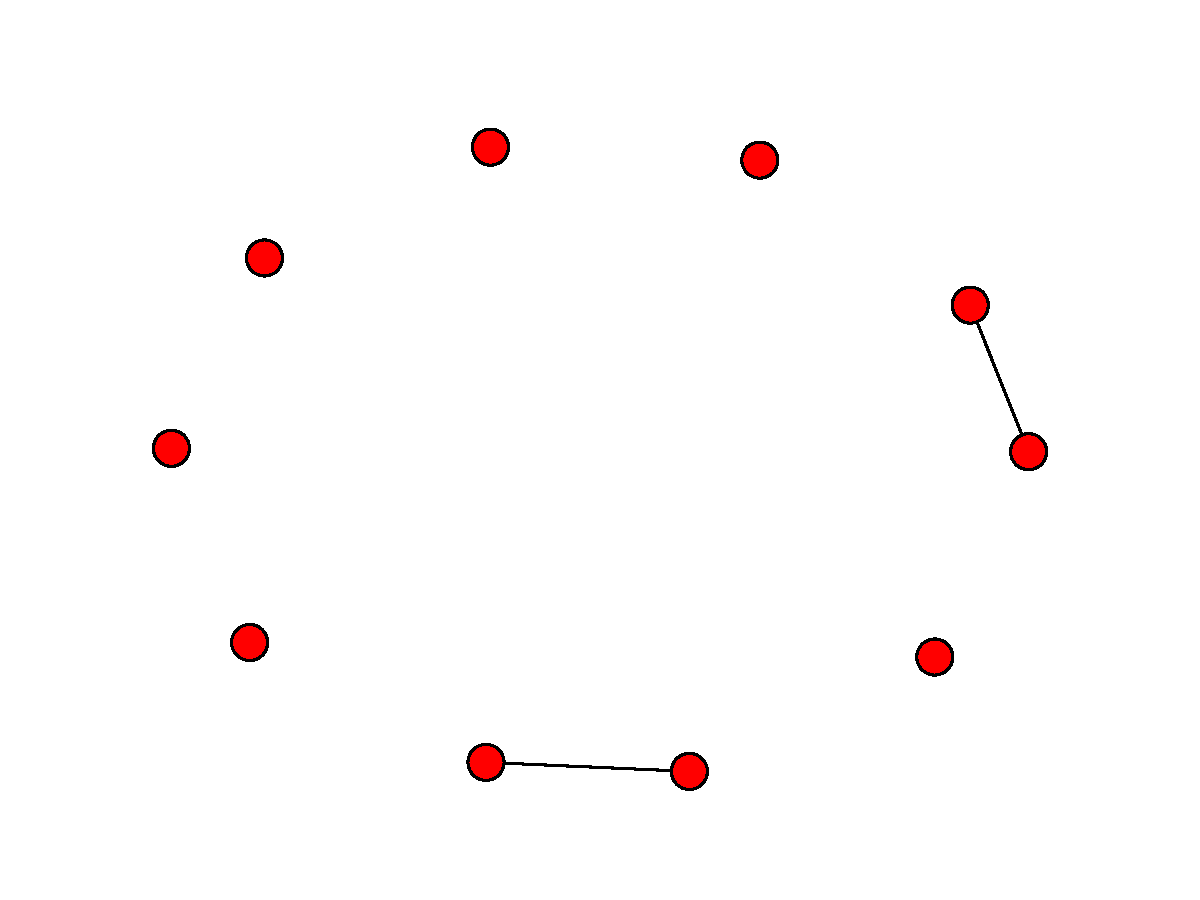
\includegraphics[width=\textwidth]{figures/ER_graph_1.pdf}
                \caption{$p=0.1$}
        \end{subfigure}
	 \begin{subfigure}[b]{0.45\textwidth}
                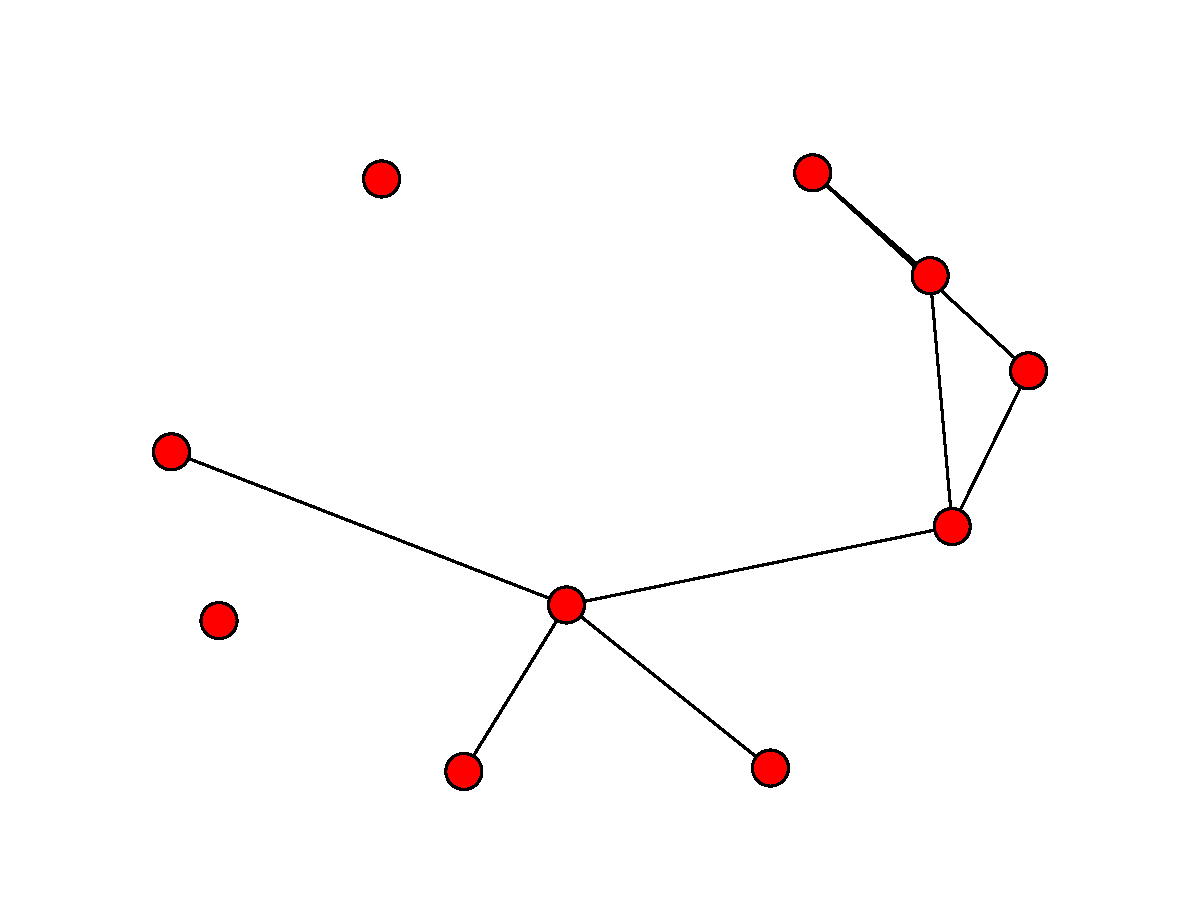
\includegraphics[width=\textwidth]{figures/ER_graph_2.pdf}
                \caption{$p=0.2$}
        \end{subfigure}
	 \begin{subfigure}[b]{0.45\textwidth}
                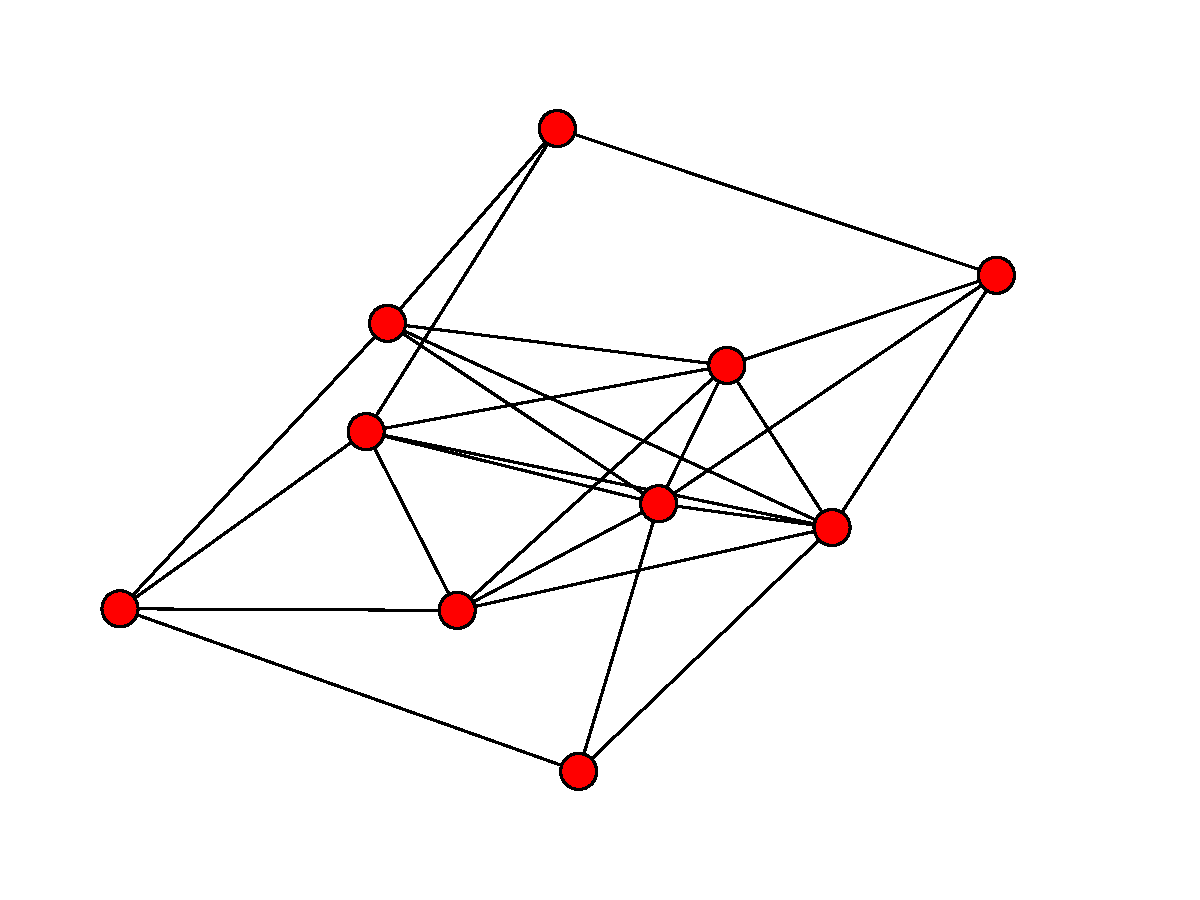
\includegraphics[width=\textwidth]{figures/ER_graph_5.pdf}
                \caption{$p=0.5$}
        \end{subfigure}
	 \begin{subfigure}[b]{0.45\textwidth}
                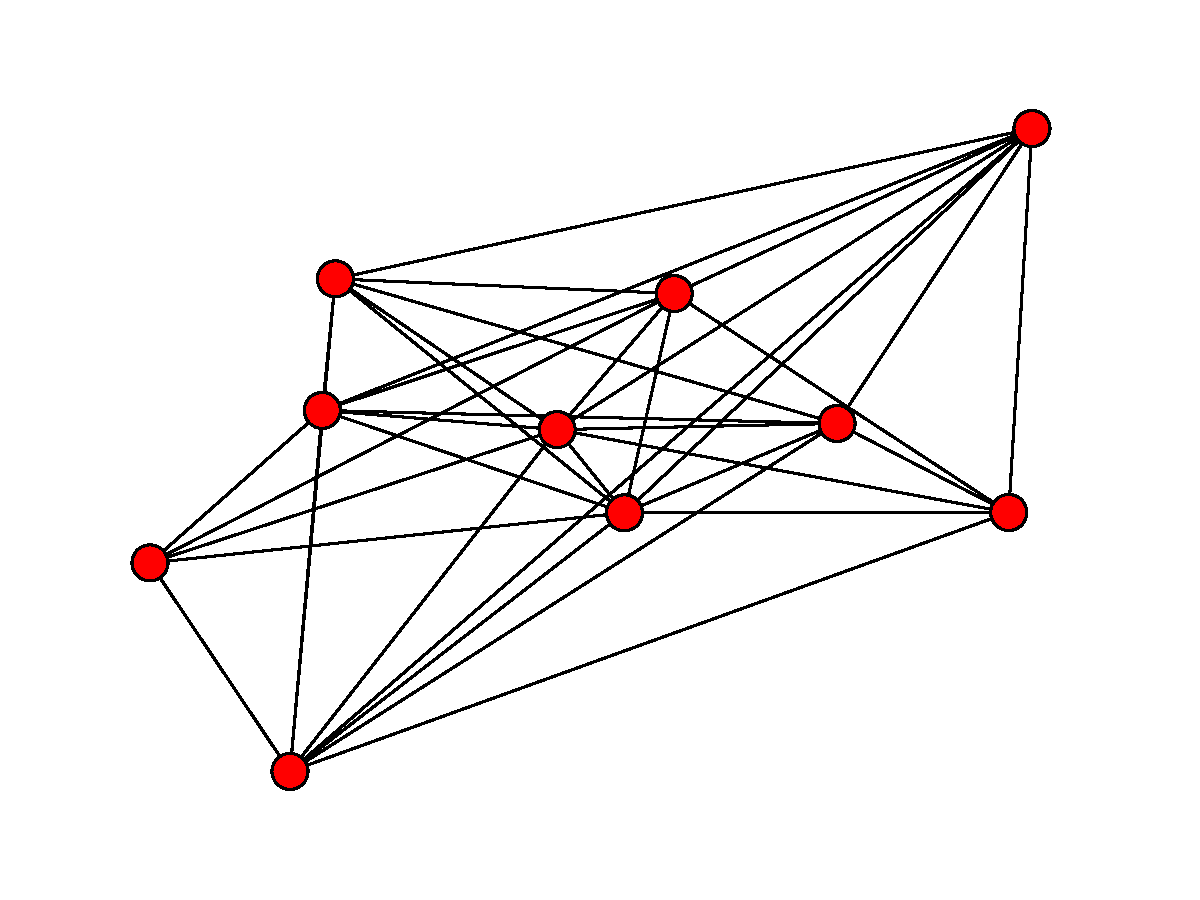
\includegraphics[width=\textwidth]{figures/ER_graph_8.pdf}
                \caption{$p=0.8$}
        \end{subfigure}
\end{center}
\caption{Examples of Erdos-Renyi graphs for various $p$}
 \label{er_ex}
\end{figure}

In our learning setting, this corresponds to the fact that when an action is chosen, other actions independently reveal their losses with a constant probability $p$.

\subsubsection{Barabási-Albert}
A Barabási-Albert (BA) graph is constructed dynamically by linking a new node to pre-existing nodes, with a probability linear in the degree of these nodes. As such, a BA graph is parametric, with parameters $m$ and $m0$, namely the number of links a node creates when joining the network, and the size of the starting graph.

These graphs are scale-free, meaning that as they grow, their degree distribution follows a power law :
$$P(k) \sim k^{-3}~\text{as}~N\rightarrow \infty$$

There are several ways to add nodes to a Barabási-Albert network. We chose to add exactly $m$ edges for each node we added, leading to the exemples of graphs in figure~\ref{ba_ex}.

\begin{figure}[h!]
\begin{center}
        \begin{subfigure}[b]{0.3\textwidth}
                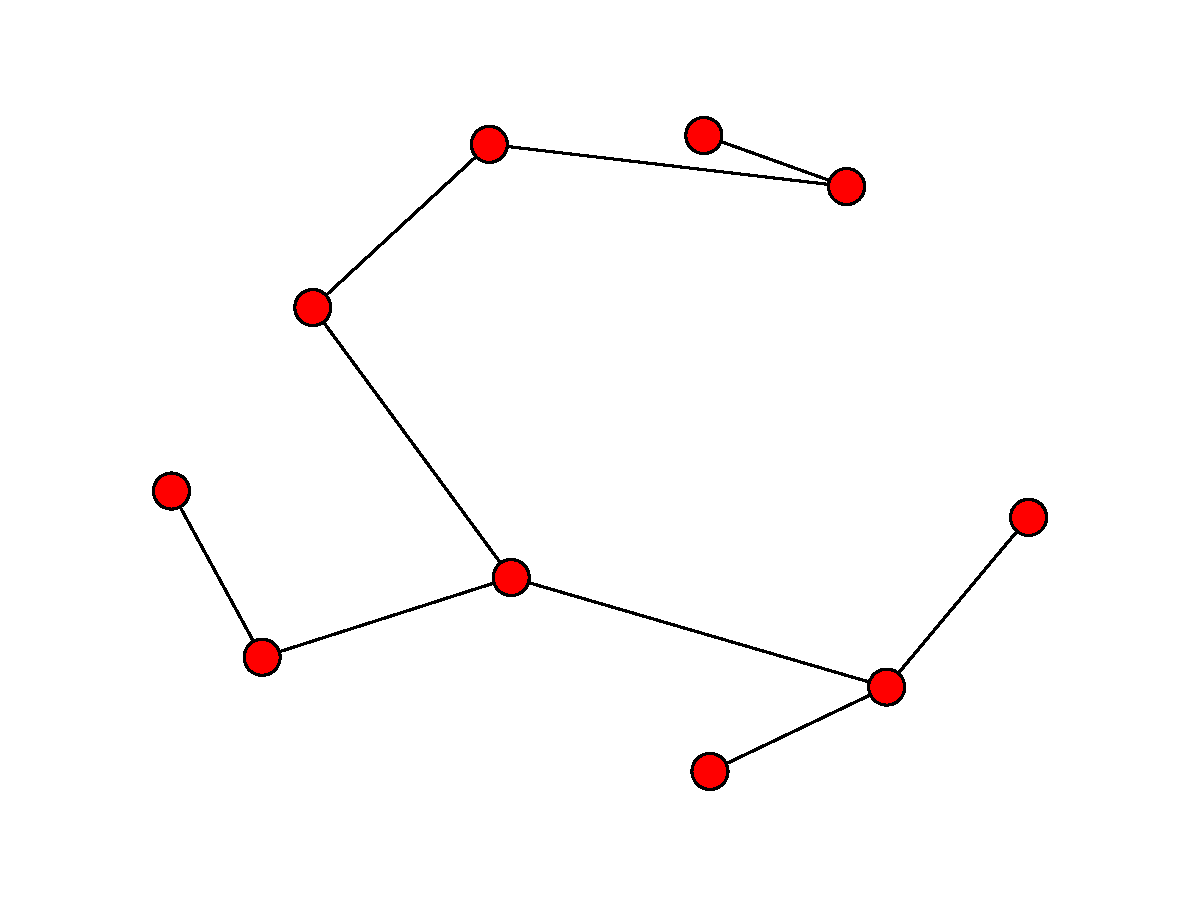
\includegraphics[width=\textwidth]{figures/BA_graph_1.pdf}
                \caption{$m=1$}
        \end{subfigure}
	 \begin{subfigure}[b]{0.3\textwidth}
                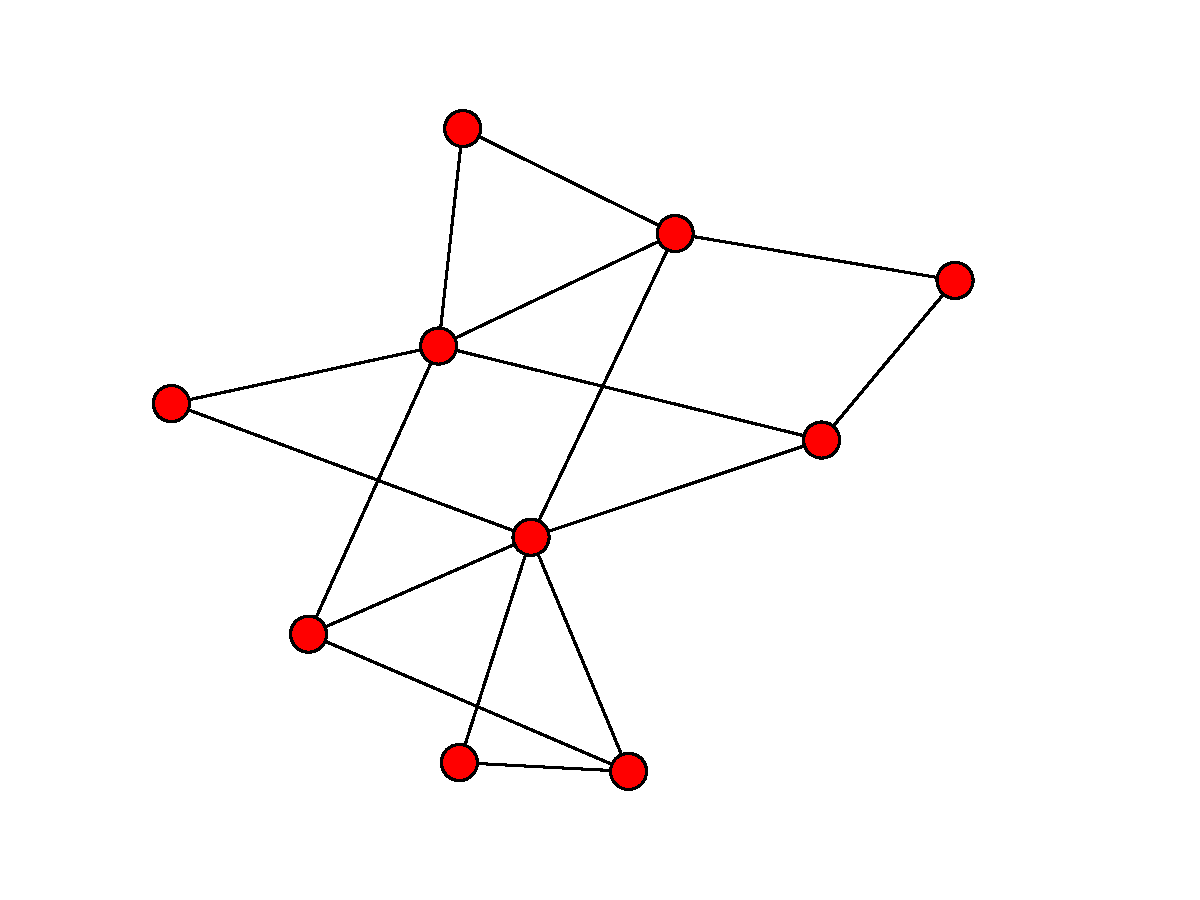
\includegraphics[width=\textwidth]{figures/BA_graph_2.pdf}
                \caption{$m=2$}
        \end{subfigure}
	 \begin{subfigure}[b]{0.3\textwidth}
                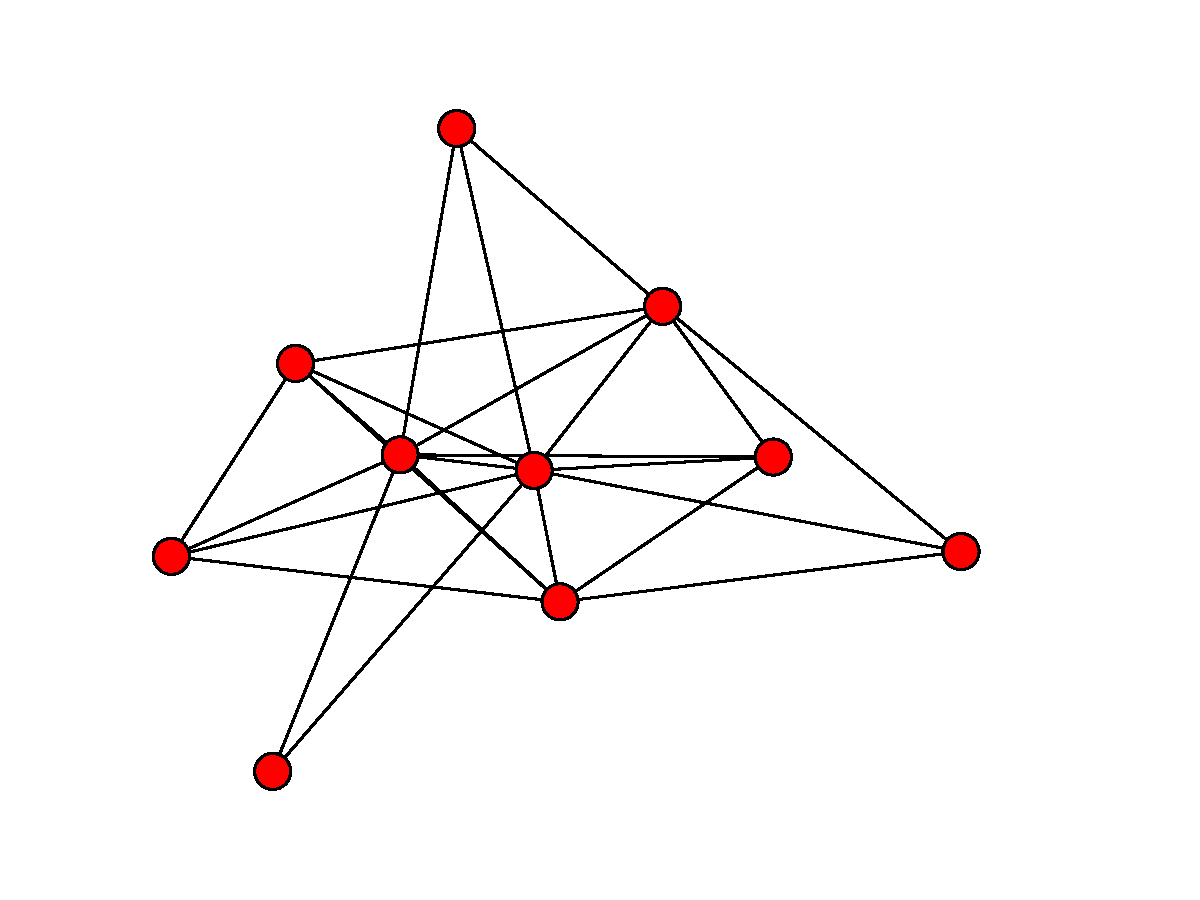
\includegraphics[width=\textwidth]{figures/BA_graph_5.pdf}
                \caption{$m=5$}
        \end{subfigure}
\end{center}
\caption{Examples of Barabási-Albert graphs.}
 \label{ba_ex}
\end{figure}
Barabási are quite good at modeling preferential attachment in social networks. [REF NEEDED]


\subsection{Objectives of our work}

In this project, we have worked on two different aspects of the topic. It is mostly based on the most recent results by Valko et al. (2015, under review).

 The first one was to experimentally compare and evaluate algorithms in the case of Erdos Renyi graphs with unknown edge distribution. The main challenge we have encountered about this is the computation time, that has prevented us to explore the performance in large scale (more than $500$ nodes) problems. At this scale, reducing the variance for the losses of the worst arms takes a long time, leading to linear cumulated regrets on a horizon smaller than $10^5$ iterations.

A second line of research is to explore an extension (or adaptation) of the EXP3 algorithm with losses adapted to random Barabasi-Albert graphs.

\section{ER graphs}
\subsection{Idea of \textsc{DuplExp3} algorithm}
Valko et al. have developed an algorithm to learn in the bandit with side informations context without any prior knowledge on the graph, including the parameter of the graph $p$. The main trick used is to directly estimate the quantity $\frac{1}{p_{t,i}+(1-p_{t,i})r}$ through two independent geometric variable~\cite{neu2013efficient}. This allows to get good loss estimate, and with an adequately tuned learning rate, to achieve a regret of $O(\sqrt{(T/r)\log N})$ for high $r$.


In the general case, a separate algorithm to obtain a lower bound on $r$ is obtained. In case $r$ is to low to obtain a reasonable estimate of $\frac{1}{p_{t,i}+(1-p_{t,i})r}$, several iterations of the previously described algorithm are grouped together. Indeed, for a too low $r$, there might not be enough samples in a single round to guarantee a reliable estimation. 


\subsection{Examples of regret curves on ER graphs and comparison with EXP3}

First of all, we verify that our implementation of the algorithm DuplExp3 fares well against EXP3~\cite{auer2002nonstochastic} on a reasonably sized graph. Fig~\ref{duplexp3vsexp3ER} shows the lower cumulated regret obtained by DuplExp3.

To achieve this, we have implemented both EXP3 (used with parameters $\gamma=\eta=0.01$) and the universal DuplExp3 algorithm (for any value of $r$). The losses are Bernoulli variables, one with parameter $0.5$, and others with parameter $0.5 + \epsilon$ (we have set $\epsilon = 0.1$). In the EXP3 setting, the weights are updated for all observed losses. Both algorithms are run 100 times, and the cumulated regret is averaged over all the runs.

As the computations time is prohibitive, it was not possible in this work to test on graphs with more nodes, but behaviour on small graphs already shows some interesting properties on the regret curves. 

\begin{figure}[h!]
\centering
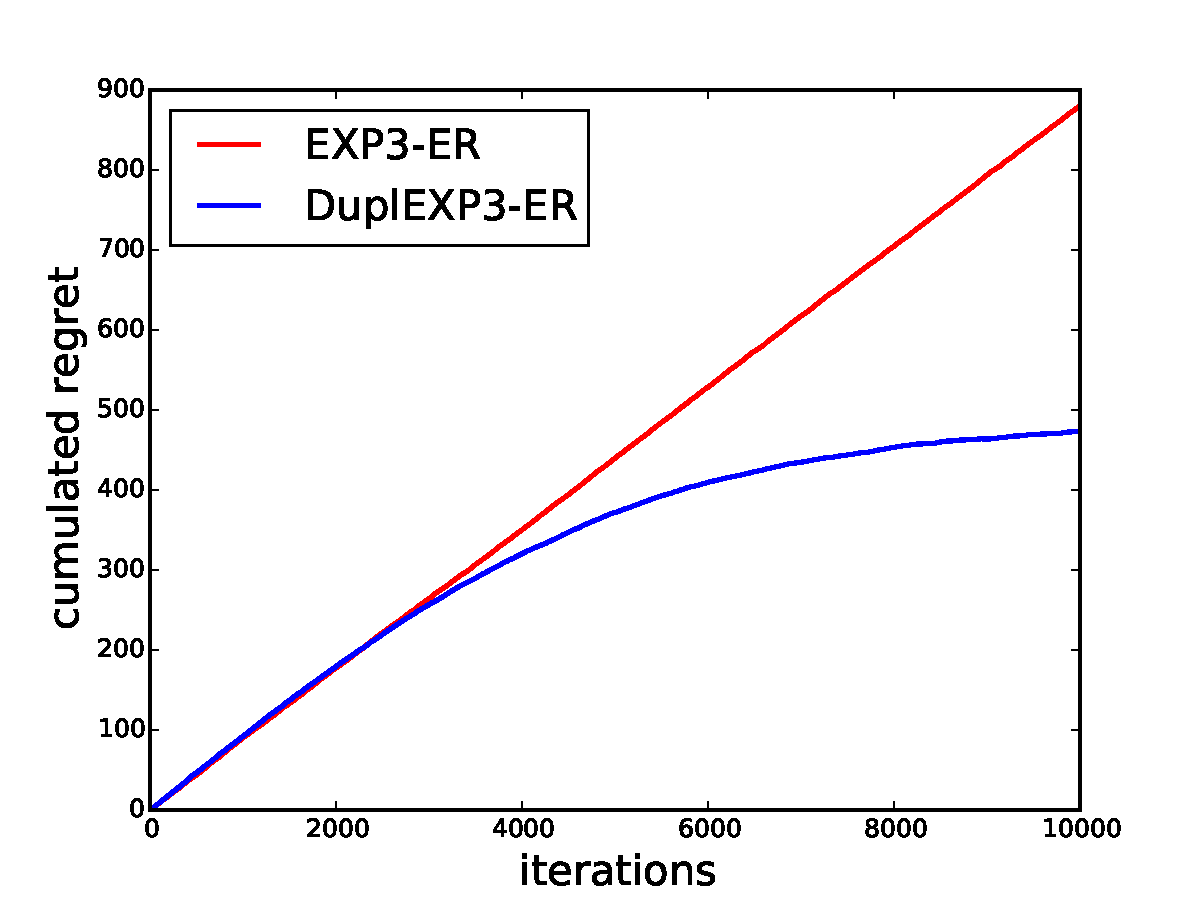
\includegraphics[height=6cm]{figures/50new_dupl_big_r05.pdf}
\caption{Comparison of cumulated regret over iterations for EXP3 and DuplExp3 algorithms for and ER graph of 50 nodes with parameter $p=0.5$ (repeated 100 times)}
\label{duplexp3vsexp3ER}
\end{figure}

\section{BA graphs}
\subsection{Empirical properties of BA graphs}
\paragraph{Independence Number}
Considering the induced hub structure on BA graphs, we conjecture that for the same edge proportion, the mean independence number is higher for BA graphs than for ER graphs.  Our conjecture holds true empirically, as shown in Fig~\ref{mean_alpha_ba_er}. Having a higher average independence number affects the bound shown by [REF NEEDED], and let's us infer that DuplExp3 won't work as well on BA graphs as it does on ER graphs.

\begin{figure}[h!]
\centering
 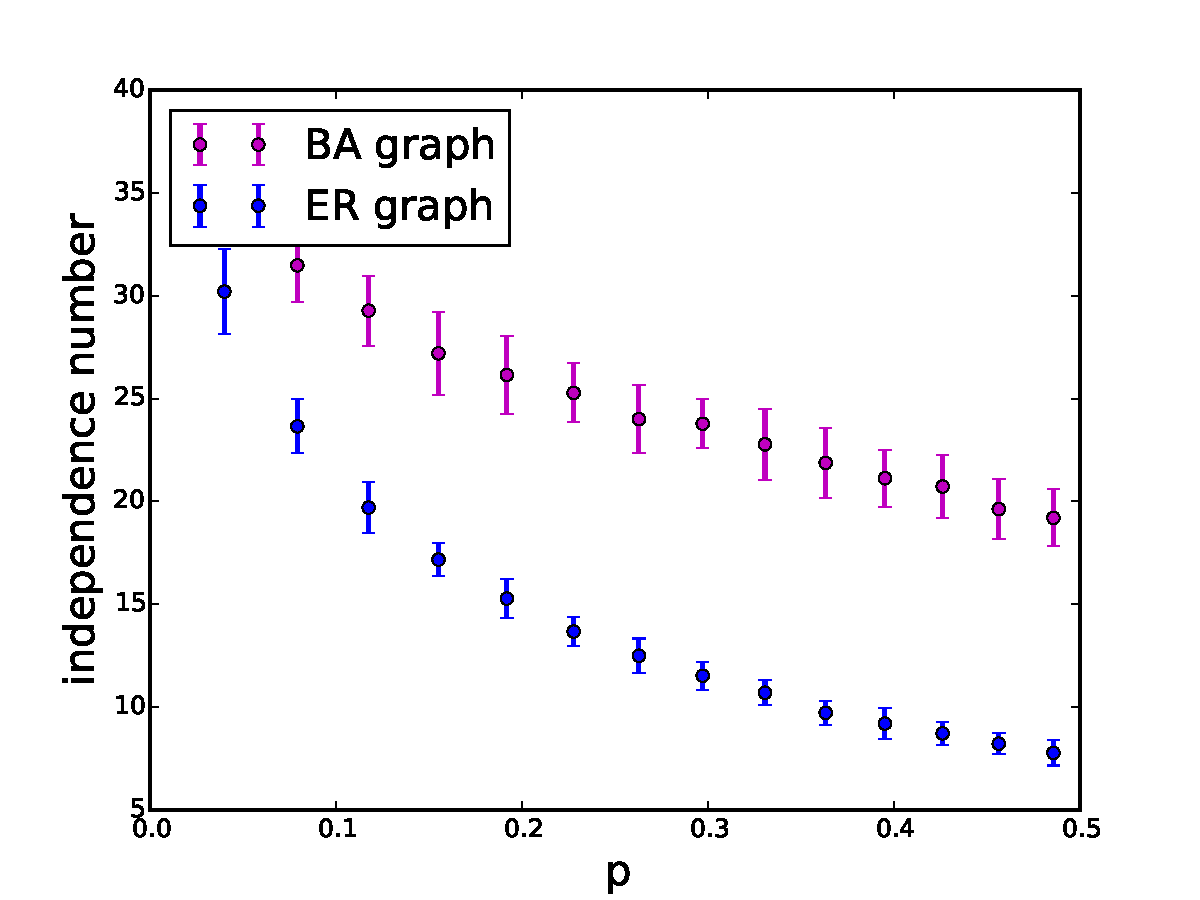
\includegraphics[height=7cm]{figures/independance_number_com.pdf}
 \caption{Average independence number for ER and BA graphs with equal edge proportion. We can see that the independence number of BA graphs stays above the independence number for ER graphs. The points and error bars correspond respectively to the mean and standard deviation obtained for 40 independant draws of a random graph of 50 nodes for each edge proportion, with varying edge proportion.}
 \label{mean_alpha_ba_er}
\end{figure}

\paragraph{Estimated r}
Another conjecture is that the degree disribution for BA Graphs will lead the estimation process in DuplExp3 astray. Leading to worse results.


proof of $\E[M_t] \leq \frac{1}{p}$ ??
si pas proof et figure : figure
si rien ... rien


\subsection{Algorithms on BA graphs}
\subsubsection{Asymptotic regime}
As the number of nodes in a BA graph grows, the degree distribution becomes more and more independent of its initial states and parameter. We can then compute the revelation probability for an arm :
$$r = \frac{\E[degree]}{N-1} = \frac{\pi^2}{6*(N-1)}$$
By setting the losses of EXP3 to be 
$$\hat{l}_{i,t} = \frac{O_{i,t}l_{i,t}}{p_{i,t}+(1-p_{i,t})r}$$
We then get non-biased loss estimates for the asymptotic regime.

\subsubsection{Finite regime}
\paragraph{DuplExp3 on BA Graphs}
To show that the conjecture on higher average independence numbers, and wrong revelation probability estimations indeed lead to an increased regret for \emph{DuplExp3}, we compare regrets of our implementations on ER and BA graphs with the same proportion of edges. Results are shown in Fig~\ref{dupl_er_ba}. As expected, DuplExp3 doesn't work as well on BA graphs.

\begin{figure}[h!]
\centering
 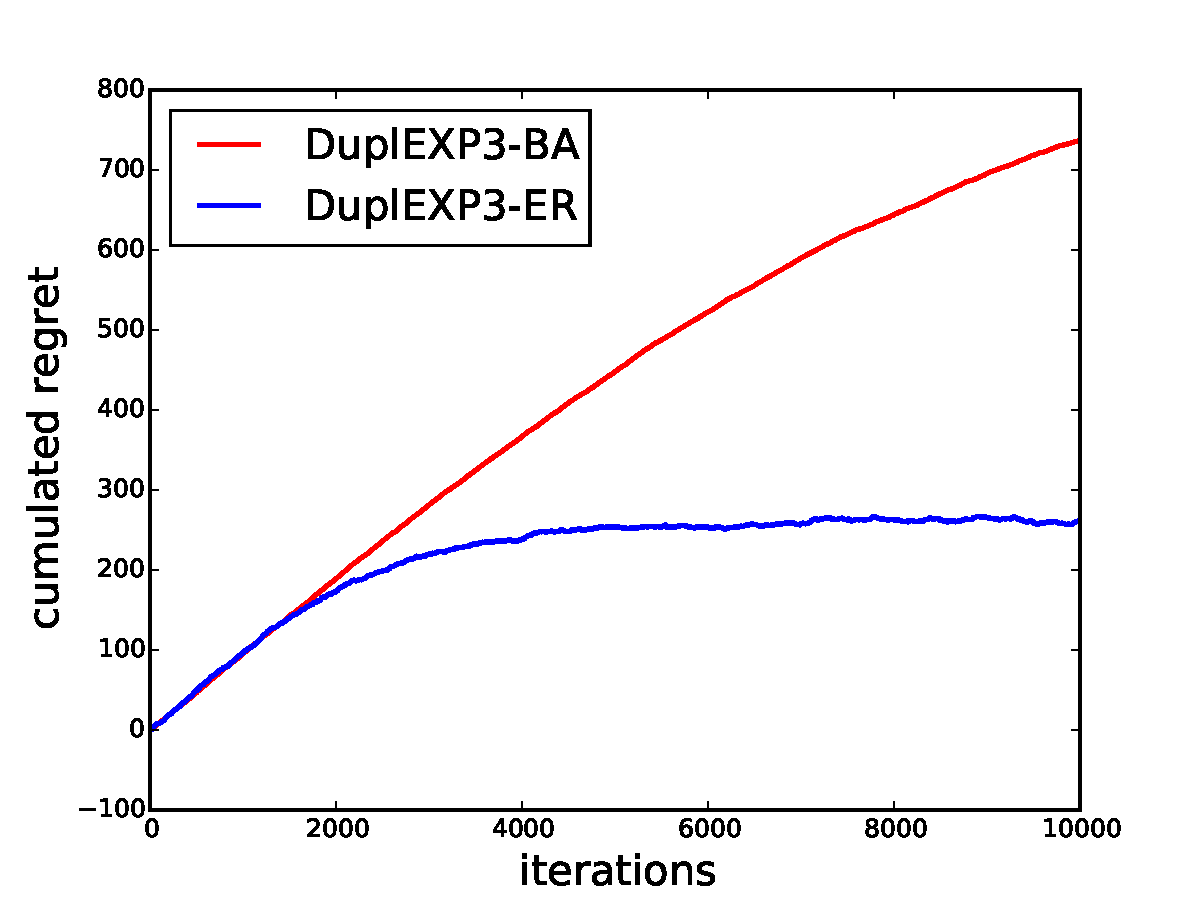
\includegraphics[height=7cm]{figures/50compare_dupl_er_ba.pdf}
 \caption{Average regret for DuplExp3 on BA and ER graphs with the same proportion of edges.}
 \label{dupl_er_ba}
\end{figure}

We have tried to implement an adaptation of DuplEXP3 where the \emph{revelation probabillity} is known and computed using the true degree distribution of the BA graph to small ($50$ nodes) BA graphs, which led to the plot in Fig~\ref{dupl_ba_finite_ba}.

\begin{figure}[h!]
\centering
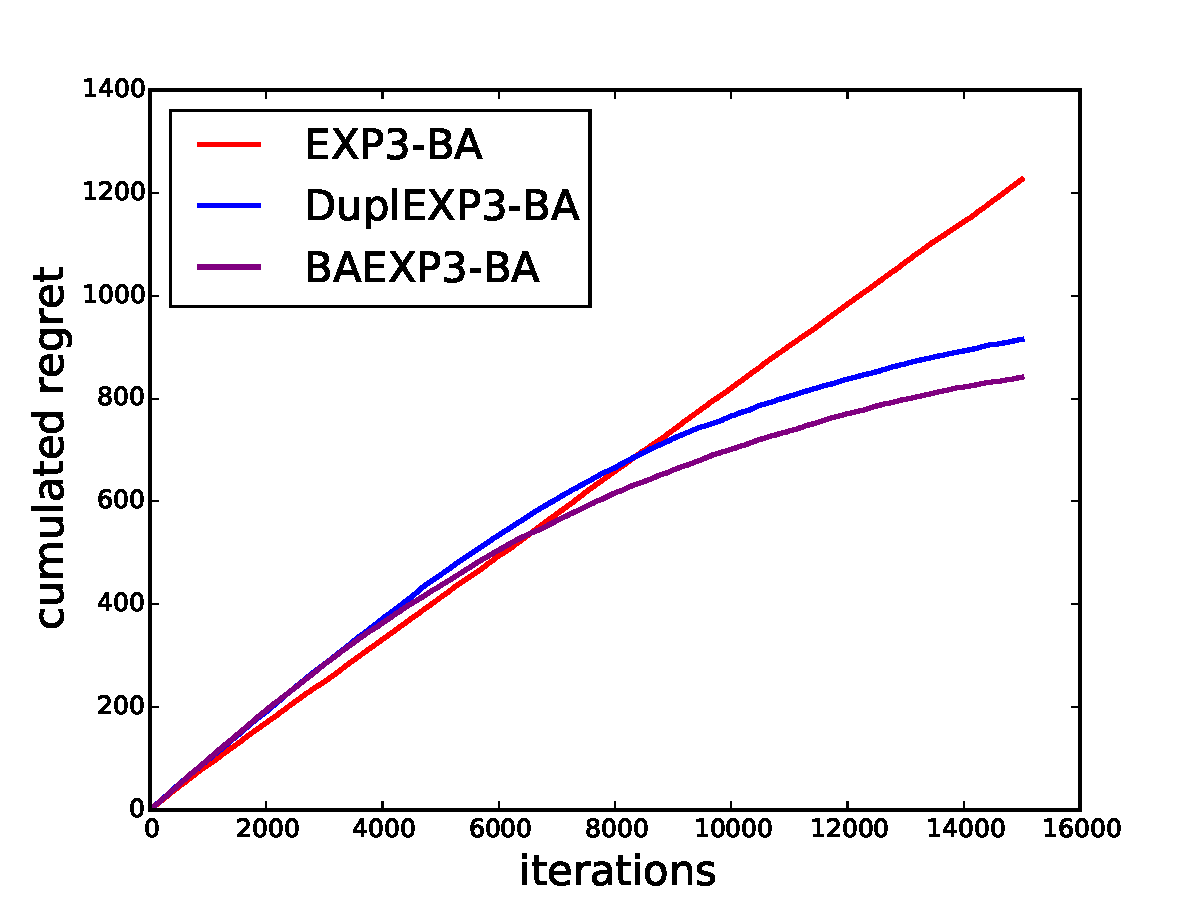
\includegraphics[height=7cm]{figures/50Kestim_BAdupl_big.pdf} % computed on godzilla
 \caption{Regret for multiple algorithms on BA graphs of size $50$, with $m=7$.}
 \label{dupl_ba_finite_ba}
\end{figure}

 It is interesting to notice that the cumulated regret is slightly smaller than with the actual DuplEXP3 algorithm, but not so much smaller. This indicates that the loss of performance due to not having the full knowledge of $r$ in BA graphs is small; in other words, DuplEXP3 performs well at taking $r$ into account (even though $r$ is never explicitely estimated). 

Comparison with the performance on ER graphs (Figure~\ref{dupl_er_ba}) can suggest that $r$ (and hence the idea of  DuplEXP3) is not so relevant to leverage side observation in BA graphs. In our current setting where the graph is unknown and changes at each iteration, it is hard to think of other quantity that could perform better. As one of the advantages to use BA graphs is to be closer to the behavior of social networks, it could be interesting to consider more stability of the graph structure over iterations, e.g. the nodes with high degree could remain so over iterations. 




\section{Conclusion}
We studied an alternative framework for bandit learning. We explored how the type of random graph affected the algorithm's results. DuplExp3 does a good job estimating the revelation probability, even when graphs are not from the Ernos-Renyi distribution. We empirically showed that average independence number for BA graphs was higher than those of ER graphs. This difference may explain the difference of performance for DuplExp3 on graphs that share the same edge proportion, but with different structure. It is hard in our setup to really exploit the distinctive degree distribution of BA graphs, since a new graph is created by the environment at each iteration. In a setup closer to the reality of social networks, it might be interesting to study regret bounds when the graph is known, or follows the BA evolution at each iteration. 

\bibliographystyle{plain}
\bibliography{bilbio}


\end{document}